% Adicionales
%\begin{additional} 
%\section{Capítulo Adicional que no es apéndice}
%\end{additional}

% Apéndices
\begin{appendix} 
\section{Glosario}

\begin{enumerate}
\item{\textbf{Etendue}}\\
\label{a1:etendue}



\item{\textbf{PSF}}\\
\label{a1:psf}
Corresponde a la respuesta instrumental a una fuente de luz puntual, cuya radiaci\'on debe atravesar la atm\'osfera terrestre y los lentes del telescopio. La distorsi\'on puede ser interpretada como la convoluci\'on de la imagen por un kernel. \cite{huentelemu}. Ver imagen \ref{fig:a1}

\begin{figure}[h]
\centering
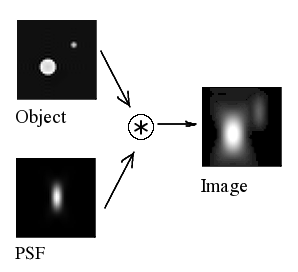
\includegraphics[scale=.5]{images/psf}
\caption{Ejemplo de distorsi\'on de una fuente al aplicar un kernel de PSF espec\'ifico. El resultado se observa en el cuado \textit{Image}.}
\label{fig:a1}
\end{figure}

\item{\textbf{Airmass}}\label{ap:airmass}\\
Es el largo del camino de que le toma a los rayos de una cuerpo celeste atravesar la atm\'osfera. A medida que los rayos van penetrando la atm\'osfera estos se van atenuando por la absorci\'on y el proceso conocido como scattering. 
\end{enumerate}
\bigskip

\section{Refactoring}
\subsection{Librer\'ias usadas para el refactoring}
\label{subs:a0}
Versi\'on de Python: 3.5
\begin{itemize}
\item \textbf{\texttt{pandas}: 0.24.4}
\item \textbf{\texttt{matplotlib}: 2.2.2}
\item \textbf{\texttt{numpy}: 1.13.3}
\item \textbf{\texttt{mahotas}: 1.4.4}
\item \textbf{\texttt{astropy}: 3.0.2}
\end{itemize}
\subsection{Rutas a directorios y expresiones regulares de archivos}
\label{subs:des_rutas}
Los campos se describen a continuaci\'on:
\begin{itemize}
\item \textbf{\texttt{maskDir}}: Directorio donde se almacenan las im\'agenes m\'ascara (im\'agenes que identifican p\'ixeles que no deben ser considerados).
\item \textbf{\texttt{scienceDir}}: Directorio donde se almacenan las im\'agenes cient\'ificas (im\'agenes base ya preprocesadas).
\item \textbf{\texttt{diffDir}}: Directorio donde se almacenan las im\'agenes de diferencia (resta entre las im\'agenes base y cient\'ifica).
\item \textbf{\texttt{psfDir}}: Directorio donde se encuentran los modelos de psf (ap\'endice \ref{a1:psf}) usados para la determinaci\'on del flujo.
\item \textbf{\texttt{invDir}}: Directorio que guarda las im\'agenes correspondientes a la varianza inversa (\textit{peso} de cada pixel en t\'erminos de ruido: a menor peso, mayor ruido).
\item \textbf{\texttt{afluxDir}}: Directorio que contiene los archivos de extensi\'on \texttt{NPY} dentro de los cuales se guarda el valor de la variable \texttt{aflux}.
\item \textbf{\texttt{maskRegEx}}: Expresi\'on regular con la que es posible identificar el nombre de las im\'agenes m\'ascara en disco siguiendo el path \texttt{maskDir}.
\item \textbf{\texttt{scienceRegEx}}: Expresi\'on regular con la que es posible identificar el nombre de las im\'agenes cient\'ificas en disco siguiendo el path \texttt{scienceDir}.
\item \textbf{\texttt{diffRegEx}}: Expresi\'on regular con la que se identifican el nombre de las im\'agenes de diferencia en disco siguiendo el path \texttt{diffDir}.
\item \textbf{\texttt{invRegEx}}: Expresi\'on regular con la que es posible identificar el nombre de las im\'agenes de la varianza inversa siguiendo el path \texttt{invDir}.
\item \textbf{\texttt{afluxRegEx}}: Expresi\'on regular con la que se identifica el nombre de los archivos \textit{match} que contienen el valor de \texttt{aflux}. Estos archivos est\'an ubicados en el path \texttt{afluxDir}.
\item \textbf{\texttt{psfRegEx}}: Expresi\'on regular que describe el nombre de las im\'agenes que guardan el modelo de PSF en el directorio \texttt{psfDir}.
\end{itemize}

\subsection{Archivo de entrada: configuraci\'on de paths}
\label{subs:a1}
\VerbatimInput{/home/paloma/Documents/Memoria/Code/sif2/inputs/dirset_leftraru.txt}


%\section{Nueva funcionalidad}
%\subsection{Modelo de archivo de almacenamiento de resultados}
\subsection{M\'etodos}
\subsubsection{Lectura y preparaci\'on de im\'agenes}
\label{subs:a2}
A continuaci\'on se enumeran los diferentes m\'etodos que intervienen en la recolecci\'on de los datos a ser le\'idos:

\begin{itemize}
\item \textbf{\texttt{config\_reg\_expressions(semester, field, ccd)}}\\
Este m\'etodo recibe como par\'ametros strings que indiquen el semestre (\texttt{semester}), el campo (\texttt{field}) y el ccd (\texttt{ccd}) que se quiere analizar. Puede hacerse uso de los valores de las variables de instancia que la misma clase \textsc{DataPicker} recibe en su constructor. Con estos strings se establecen las rutas de los directorios de las im\'agenes y las expresiones regulares de los nombres de las mismas.
\bigskip

\item \textbf{\texttt{collect\_data()}}\\
Esta funci\'on se encarga de recolectar la ruta completa de las diferentes im\'agenes (m\'ascaras, im\'agenes cient\'ificas, de diferencia, etc.). Para esta finalidad se hace uso del m\'etodo \texttt{walking\_through\_files}. 
\bigskip

\item \textbf{\texttt{walking\_through\_files(regex, dir)}}\\
M\'etodo con el cual se recorren las rutas definidas en los pasos anteriores y se agrupan los nombres completos (directorio incluido) de las im\'agenes ubicadas en el directorio \texttt{dir} y posean un nombre de patr\'on que siga la expresi\'on regular \texttt{regex}.
\bigskip

\item \textbf{\texttt{filter\_science\_images()}}\\
Filtra im\'agenes cient\'ificas de acuerdo a su airmass (Ap\'endice  \ref{ap:airmass}), seleccionando aquellas obtenidas en fechas cuyo valor de airmass calculado es menor a 1,7. De esta secuencia de im\'agenes cient\'ificas resultante se obtiene una lista de fechas que cumplen esta condici\'on, medidas en t\'erminos de \textit{d\'ia juliano modificado} o \textit{Modified Julian Date} (MJD) de tipo punto flotante. Estos valores son ordenados de forma creciente.%las fechas en que las observaciones fueron hechas en t\'erminos de \textit{d\'ia juliano modificado} o \textit{Modified Julian Date} (MJD) como variables de punto flotante.
\bigskip

\item \textbf{\texttt{select\_fits(dir)}}\\
Selecciona y ordena los elementos de la lista de im\'agenes de formato \textsc{fits} del directorio \texttt{dir} usando la lista de MJDs (guardada en la variable de instancia \texttt{mjd} de la clase) generada en \texttt{filter\_science\_images()} escogiendo s\'olo aquellas cuyas fechas correspondan a las fechas indicadas.  %cronol\'ogico (i.e. de acuerdo a la secuencia de MJD encontrada en \texttt{filter\_science\_images()}).
\bigskip

\item \textbf{\texttt{select\_npys(dir, ref\_dir, init\_index, n\_pos, rest\_len)}}:\\
Debido a que los archivos de extensi\'on NPY no poseen la variable MJD en su estructura (en los archivos \textsc{fits} encontramos este valor en el header de la imagen) deben de filtrarse de forma diferente. Para este caso el filtrado de este tipo de archivos se lleva a cabo a trav\'es de la revisi\'on de sus nombres, ya que comparten patrones con los nombres de ciertas im\'agenes \textsc{fits}. Por ejemplo, los nombres de las im\'agenes de PSF, de formato NPY, poseen similitud con los nombres de las im\'agenes \textsc{fits} de diferencia; igualmente los archivos \texttt{aflux} de formato NPY poseen parecidos en sus nombres con las im\'agenes cient\'ificas. Esta similitud es medida a trav\'es de un substring diferente para cada tipo de archivo NPY, definido por la posici\'on inicial \texttt{init\_index}, en el nombre del archivo \textsc{fits} y largo \texttt{rest\_len}. \texttt{n\_pos} indica la posici\'on de un car\'acter espec\'ifico `` \_ '' en dicho substring para validar esta comparaci\'on.

\end{itemize}


\subsection{Diccionario de par\'ametros y umbrales}
\label{subs:a3}
El diccionario de umbrales y par\'ametros de configuraci\'on contiene la siguiente lista de valores:

\begin{itemize}
\item \texttt{imgHeight}: Altura de las im\'agenes cient\'ificas en p\'ixeles. Esta dimensi\'on se propaga al resto de im\'agenes y matrices. Las im\'agenes usadas en este trabajo poseen una altura de 4094 p\'ixeles. 
\item \texttt{imgWidth}: Ancho de las im\'agenes cient\'ificas en p\'ixeles. Esta dimensi\'on se propaga al resto de im\'agenes y matrices, y en este trabajo las respectivas im\'agenes poseen un ancho de 2046.
\item \texttt{filter}: Tipo de filtro (\texttt{basic}, \texttt{mcc} o \texttt{ukf}).
\item \texttt{results}: Directorio de resultados (donde se guardan las coordenadas de los candidatos encontrados junto a lista de \'epocas en que fueron detectados) en formato NPZ.
\item \texttt{init\_var}: Varianza inicial que tendr\'an las matrices de covarianza durante el proceso de estimaci\'on con los filtros de Kalman. 
\item \texttt{flux\_thresh}: Umbral para estado de flujo obtenido con Kalman. Es un valor determinado por el usuario (en este trabajo se defini\'o como 200). 
\item \texttt{flux\_rate\_thresh}: Umbral para la velocidad de flujo obtenido con Kalman. Es un valor establecido por el usuario (en este trabajo se defini\'o como 50).
\item \texttt{rate\_satu}: Tasa de saturaci\'on.
\item \texttt{sigma\_a}: Varianza de la distribuci\'on de la componente de control ($u_k$) asumiendo normalidad. Es importante al emplear los filtros b\'asico y unscented, ya que corresponde a la desviaci\'on est\'andar de la distribuci\'on normal de la aceleraci\'on originada por cambios no esperados en el modelo (lo que se puede interpretar como ``fuerzas externas'') \cite{ian}.
\item \texttt{epsilon}: Radio de error con que la estimaci\'on por filtro de Kalman de m\'axima correntrop\'ia disminuye la ganancia de Kalman. Corresponde a un criterio de detenci\'on y toma valores entre 0 y 1 (t\'ipicamente, $10^{-6}$)\cite{badong}.
\item \texttt{max\_iter}: N\'umero de iteraciones m\'aximo para el proceso de correcci\'on al usar Kalman de m\'axima correntrop\'ia. 
\item \texttt{silverman}: \textit{Entero}. Toma valor 1 en caso de considerarse, y 0 si no. Se establece si se usa o no la aproximaci\'on de Silverman para determinar ancho de banda del kernel al emplear el filtro de m\'axima correntrop\'ia.
\item \texttt{std\_factor}: Factor de incremento de sigma al usar el m\'etodo de Silverman.
\item \texttt{sigma}: Sigma usado por defecto sin Silverman en la determinaci\'on del kernel durante el proceso de correcci\'on con el Filtro de Kalman de correntrop\'ia m\'axima .
\item \texttt{beta}: Par\'ametro relacionado con la distribuci\'on del estado estimado ($x_k$). Toma valor de $\beta = 2$ para distribuciones normales.
\item \texttt{kappa}: Participa en la regulaci\'on del rango de los valores de los puntos sigma y usualmente toma valores entre 1 y 3N-1 (N corresponde al n\'umero de dimensiones)\cite{wan}. Aporta incremento adicional (ver Ecuaci\'on \ref{eq:eq21}).
\item \texttt{alpha}: Participa en la regulaci\'on del rango de los valores de los puntos sigma, y generalmente toma valores positivos menores o iguales a 1: $10^{-4} \leq \alpha \leq 1 $\cite{wan}. Incrementa el rango en un factor $\alpha$ (ver Ecuaci\'on \ref{eq:eq21}).
\item \texttt{dim}: Cantidad de componentes de estado a medir (en este programa se miden dos: flujo y su velocidad).
\end{itemize}
\subsection{Archivo de entrada: par\'ametro y umbrales}
\label{subs:settings_file}
\VerbatimInput{/home/paloma/Documents/Memoria/Code/sif2/inputs/settings_example.txt}
\subsection{Archivo de entrada: lista de campos, CCDs y semestres (incluye algunas coordenadas)}
\label{subs:sn_list}
\VerbatimInput{/home/paloma/Documents/Memoria/Code/sif2/inputs/hits15.csv}

\subsection{M\'etodos de la clase \textsc{RoutineHandler}}
\label{subs:a4}
\begin{itemize}
\item \texttt{process\_settings():}\\
En este m\'etodo se lee el archivo de diccionario de umbrales y par\'ametros con los que se configurar\'a la toma de decisiones del programa.
\bigskip

\item \texttt{retrieve\_kalman\_filter(kalman\_string):}\\
Corresponde a un m\'etodo auxiliar que es invocado desde \texttt{process\_settings} con el que se crea una instancia del filtro de Kalman a partir de la lectura del archivo de valores, de acuerdo al valor definido por el usuario. Los tres strings v\'alidos para la construcci\'on de una instancia son: `basic', `mcc' y `ukf'. Si se entrega otro tipo de string, se levanta un error.
\bigskip
  
\item \texttt{iterate\_over\_sequences(check\_found\_objects):}\\
Recorre la lista de campos, CCDs y semestres entregada al programa con la consiguiente llamada a \texttt{routine}. Recibe como par\'ametro el argumento \texttt{check\_found\_objects} con el cual se indica si se quiere analizar resultados obtenidos anteriormente (candidatos encontrados), y que es entregado al m\'etodo \texttt{routine} descrito a continuaci\'on.
\bigskip

\item \texttt{routine(semester, field, ccd, results\_path, check\_found\_objects, last\_mjd):}\\
Comprende la rutina principal del programa, es decir, el an\'alisis de las observaciones de un semestre, campo y CCD espec\'ifico. El argumento \texttt{check\_found\_objects} es un boolean e indicar\'a el modo de ejecuci\'on del m\'etodo: si es falso, s\'olo guardar\'a las coordenadas de los candidatos encontrados (si no encontr\'o nada, entonces se guarda una lista vac\'ia) adem\'as de las \'epocas en que fueron detectados. Esta informaci\'on se guarda en un arreglo de diccionarios. Si \texttt{check\_found\_objects} es verdadero, entonces cargar\'a resultados anteriores del directorio de resultados (configurado en \texttt{process\_settings}) para estudiar la presencia de los candidatos encontrados en caso de existir.
\end{itemize}  
\bigskip
%\section{Unit-tests}
%\subsection{Refactoring}
\pagebreak

\section{Detecci\'on usando pipeline original}
\begin{table}[h!]
\small
\centering
\caption{Resultados de \'epocas de detecci\'on en t\'erminos de MJD de las 93 supernovas del conjunto de 2015 de HiTS, usando los filtros implementados originalmente (b\'asico y de correntrop\'ia m\'axima).}
\begin{tabular}{|l|r|r|}
\hline
\textbf{\'Ind.} & \textbf{B\'asico} & \textbf{MCC}   \\
\hline
1&57072,19 & 57072,19 \\
2&-             & -             \\
3&57075,15 & 57075,15 \\
4&57075,21 & 57075,21 \\
5&57072,24 & 57072,24 \\
6&-             & -             \\
7&-             & -             \\
8&57075,10 & 57075,10 \\
9&57075,22 & 57075,22 \\
10&57077,11 & 57077,11 \\
11&57075,20 & 57075,20 \\
12&57072,21 & 57072,21 \\
13&57077,15 & 57077,15 \\
14&-             & -             \\
15&57077,11 & 57077,11\\
16&57077,09 & 57077,09\\
17&57077,11 & 57077,11 \\
18&57090,23 & 57090,23 \\
19&-             & -             \\
20&57077,12   & 57077,12  \\
21&-             & -             \\
22&57077,12 & 57077,12 \\
23&-             & -             \\
24&57077,08  & 57077,08   \\
25&57075,25 & 57075,25 \\
26&-             & -             \\
27&57077,17 & 57077,17 \\
28&-             & -             \\
29&-             & -             \\
30&57072,35 & 57072,35 \\
31&-             & -             \\
32&57075,21 & 57075,21 \\
33&-             & -             \\
34&-             & -             \\
35&-             & -             \\
36&57080,11 & 57080,11 \\
37&57075,21 & 57075,21 \\
38&-             & -             \\
39&-             & -             \\
40&-             & -             \\
41&-             & -             \\
42&-             & -             \\
43&57090,22 & 57090,22\\
44&-             & -             \\
45&-             & -             \\
46&-             & -             \\
47&57075,20 & 57075,20 \\\hline
\end{tabular}
\quad
\begin{tabular}{|l|r|r|}
\hline
\textbf{\'Ind.} & \textbf{B\'asico} & \textbf{MCC} \\
\hline
48&57080,17 & 57080,17 \\
49&57090,24 & 57090,24 \\
50&57075,21 & 57075,21 \\
51&-             & -             \\
52&-             & -             \\
53&-             & -             \\
54&-             & -             \\
55&-             & -             \\
56&57075,11  & 57075,11  \\
57&57095,20 & 57095,20 \\
58&-             & -             \\
59&57095,20 & 57095,20\\
60&-             & -             \\
61&-             & -             \\
62&57095,16 & 57095,16\\
63&-             & -             \\
64&-             & -             \\
65&-             & -             \\
66&-             & -             \\
67&-             & -             \\
68&-             & -             \\
69&-             & -             \\
70&-             & -             \\
71&-             & -             \\
72&-             & -             \\
73&-             & -             \\
74&-             & -             \\
75&-             & -             \\
76&-             & -             \\
77&-             & -             \\
78&-             & -             \\
79&-             & -             \\
80&-             & -             \\
81&-             & -             \\
82&-             & -             \\
83&-             & -             \\
84&-             & -             \\
85&-             & -             \\
86&57080,20 & 57080,20 \\
87&-             & -             \\
88&-             & -             \\
89&-             & -             \\
90&-             & -             \\
91&NaN           & NaN           \\
92&NaN           & NaN           \\
93&NaN           & NaN          \\\hline
\end{tabular}
\label{ap:tab1}
\end{table}
\pagebreak


\section{Detecci\'on usando pipeline refactorizada}
\label{ap:pip_ref}
\begin{table}[h!]
\small
\centering
\caption{Resultados de \'epocas de detecci\'on en t\'erminos de MJD de las 93 supernovas del conjunto de 2015 de HiTS, usando los filtros refactorizados (b\'asico y de correntrop\'ia m\'axima).}
\begin{tabular}{|l|r|r|}
\hline
\textbf{\'Ind.} & \textbf{B\'asico} & \textbf{MCC} \\\hline
1& 57072,19   & 57072,19   \\
2& -              & -              \\
3& 57075,15    & 57075,15     \\
4& -   & -   \\
5& 57072,24   & 57072,24   \\
6& 57077,09   & 57077,09   \\
7& -              & -              \\
8& 57075,10   & 57075,10   \\
9& 57075,22   & 57075,22   \\
10& 57077,11   & 57077,11   \\
11& 57075,20    & 57075,20    \\
12& 57072,14   & 57072,14   \\
13& 57077,15   & 57077,15   \\
14& -    & -    \\
15& 57077,11   & 57077,11   \\
16& 57077,09   & 57077,09   \\
17& 57077,11   & 57077,11   \\
18& -   & -   \\
19& -              & -              \\
20& 57077,18   & 57077,18   \\
21& 57077,12   & 57077,18   \\
22& 57077,12  & 57077,12   \\
23& -              & -              \\
24& 57077,08    & 57077,08             \\
25& 57077,09   & 57077,09   \\
26& -   & -   \\
27& 57077,17   & 57077,17   \\
28& -              & -              \\
29& -              & -              \\
30& 57072,21   & 57072,21   \\
31& -              & -              \\
32& 57075,21   & 57075,21   \\
33& -              & -              \\
34& -              & -              \\
35& 57078,20   & 57078,20   \\
36& 57080,11   & 57080,11   \\
37& -              & -              \\
38& - & - \\
39& -              & -              \\
40& -              & -              \\
41& 57075,08     & 57075,08              \\
42& -              & -              \\
43& 57090,22   & 57090,22   \\
44& -              & -              \\
45& -              & -              \\
46& -              & -              \\
47& 57075,20   & 57075,20   \\\hline
\end{tabular}
\quad
\begin{tabular}{|l|r|r|}
\hline
\textbf{\'Ind.} & \textbf{B\'asico} & \textbf{MCC}\\\hline
48& 57080,11   & 57080,11   \\
49& 57090,24   & 57090,24   \\
50& 57077,18   & 57077,18   \\
51& 57077,13   & 57077,13  \\
52& -              & -              \\
53& -              & -              \\
54& 57095,17              & 57095,17              \\
55& -              & -              \\
56& 57075,11   & 57075,11   \\
57& 57095,20   & 57095,20   \\
58& -              & -              \\
59& -              & -              \\
60& 57095,20              & 57095,20             \\
61& -              & -              \\
62& -   & -   \\
63& -              & -              \\
64& -              & -              \\
65& -              & -              \\
66& 57095,15   & 57095,15   \\
67& -              & -              \\
68& -              & -              \\
69& -              & -              \\
70& -              & -              \\
71& -              & -              \\
72& -              & -              \\
73& -              & -              \\
74& -              & -              \\
75& -              & -              \\
76& -              & -              \\
77& -              & -              \\
78& -              & -              \\
79& -              & -              \\
80& -              & -              \\
81& -              & -              \\
82& -              & -              \\
83& -              & -              \\
84& -              & -              \\
85& -              & -              \\
86& 57090,26   & 57090,26   \\
87& -              & -              \\
88& -              & -              \\
89& -              & -              \\
90& -              & -              \\
91& NaN            & NaN            \\
92& NaN            & NaN            \\
93& NaN            & NaN           \\\hline
\end{tabular}
\label{ap:tab2}
\end{table}
\pagebreak

\section{Detecci\'on usando filtro unscented}
\begin{table}[h!]
\small
\centering
\caption{Resultados de \'epocas de detecci\'on en t\'erminos de MJD de las 93 supernovas del conjunto de 2015 de HiTS, usando el filtro unscented para una funci\'on $f(\Delta t) = \Delta t^{1.5}$ y $f(\Delta t) = \Delta t^{2}$.}

\begin{tabular}{|l|r|r|}
\hline
\textbf{\'Ind.} & \textbf{n=1.5}  & \textbf{n=2.0}  \\\hline
1     & -        & 57072,26 \\
2     & -        & -        \\
3     & -        & -        \\
4     & -        & -        \\
5     & 57072,24 & -        \\
6     & -        & -        \\
7     & -        & -        \\
8     & -        & 57077,09 \\
9     & -        & -        \\
10    & -        & -        \\
11    & -        & -        \\
12    & -        & -        \\
13    & -        & -        \\
14    & -        & -        \\
15    & -        & -        \\
16    & -        & -        \\
17    & -        & -        \\
18    & -        & -        \\
19    & -        & -        \\
20    & 57090,24 & 57090,24 \\
21    & -        & -        \\
22    & -        & -        \\
23    & -        & -        \\
24    & -        & -        \\
25    & -        & -        \\
26    & -        & -        \\
27    & -        & -        \\
28    & -        & -        \\
29    & -        & -        \\
30    & -        & -        \\
31    & -        & -        \\
32    & -        & -        \\
33    & -        & -        \\
34    & -        & -        \\
35    & -        & -        \\
36    & -        & -        \\
37    & -        & -        \\
38    & -        & -        \\
39    & -        & -        \\
40    & -        & -        \\
41    & -        & -        \\
42    & -        & -        \\
43    & -        & -        \\
44    & -        & -        \\
45    & -        & -        \\
46    & -        & -        \\
47    & -        & -        \\\hline
\end{tabular}
\quad
\begin{tabular}{|l|r|r|}
\hline
\textbf{\'Ind.} & \textbf{n=1.5} & \textbf{n=2.0}\\\hline
48    & -        & -        \\
49    & -        & -        \\
50    & -        & -        \\
51    & -        & -        \\
52    & -        & -        \\
53    & -        & -        \\
54    & -        & -        \\
55    & -        & -        \\
56    & -        & -        \\
57    & -        & -        \\
58    & -        & -        \\
59    & -        & -        \\
60    & -        & -        \\
61    & -        & -        \\
62    & -        & -        \\
63    & -        & -        \\
64    & -        & -        \\
65    & -        & -        \\
66    & -        & -        \\
67    & -        & -        \\
68    & -        & -        \\
69    & -        & -        \\
70    & -        & -        \\
71    & -        & -        \\
72    & -        & -        \\
73    & -        & -        \\
74    & -        & -        \\
75    & -        & -        \\
76    & -        & -        \\
77    & -        & -        \\
78    & -        & -        \\
79    & -        & -        \\
80    & -        & -        \\
81    & -        & -        \\
82    & -        & -        \\
83    & -        & -        \\
84    & -        & -        \\
85    & -        & -        \\
86    & -        & -        \\
87    & -        & -        \\
88    & -        & -        \\
89    & -        & -        \\
90    & -        & -        \\
91    & NaN        & NaN        \\
92    & NaN        & NaN     \\
93    & NaN        & NaN      \\\hline
\end{tabular}
\label{ap:tab3}
\end{table}

\end{appendix}

